
\section{Particle Swarm Optimization (PSO)}
\author{Paweł Jastrzębski}
\subsection{Ogólny opis algorytmu}
\par Particle Swarm Optimaliation (PSO) lub optymalizacja rojem cząsteczek jest algorytmem zaproponowanym przez Jamesa Kennedy'ego oraz Russela Eberhart'a w roku 1995. Jest to technika wzorowana na zachowaniach występujących w przyrodzie. Algorytm naśladuje inteligencje i sposób poruszania się roju owadów poszukujących pożywienia. 
\par Zachowania te są w pewien sposób upraszczane, zamiast roju owadów mamy pewną liczbę cząsteczek (agentów) poruszających się w n-wymiarowej przestrzeni. Cząsteczki przemieszczają się w różnych kierunkach poszukując optymalnego rozwiązania. Korzystają przy tym ze swoich indywidualnych doświadczeń jak i doświadczenia ogółu.
\subsection{Działanie algorytmu}
\subsubsection{Oryginalna wersja}
$\cdots$
\subsubsection{PSO w problemie układania planu}
\par Modyfikacja PSO przedstawiona w tym rozdziale została zaczerpnięta z pracy ,,Timetable Scheduling Using Particle Swarm Optimization'' \cite{pso}
\par W tym podejściu każda cząsteczka posiada dwa kompletne plany zajęć. Jeden z nich jest przeznaczony do modyfikacji w każdej iteracji algorytmu (dalej nazywany planem aktualnym). Natomiast drugi plan jest używany do zapamiętywania dotychczas najlepszego planu znalezionego przez tą cząsteczkę (dalej nazywany lokalnie najlepszym planem). Obecny jest również globalny plan, którego zadaniem jest przechowywanie najlepszego planu znalezionego kiedykolwiek przez jakąkolwiek cząsteczkę (dalej nazywany globalnie najlepszym planem).  
\par Podczas każdej iteracji poszczególne cząsteczki będą poddawane trzem zmianom. Najpierw dwie losowe lekcje z planu aktualnego zostaną ze sobą zamienione. Potem jedna lekcja z lokalnie najlepszego planu zostanie skopiowana do aktualnego planu. Na koniec skopiujemy jedną lekcje z globalnie najlepszego planu do aktualnego planu. Kopia lekcji z innego planu wykonywana jest w następujący sposób. Wybierana jest lekcja z innego planu. Odszukujemy miejsce gdzie jest ta lekcja w aktualnym planie. Zamieniamy odszukaną lekcje z lekcją, która jest w miejscu do którego chcemy ją skopiować. 
\par Cały algorytm zaczynamy od stworzenia populacji dwudziestu cząsteczek. Każda z nich będzie posiadała losowo wygenerowany plan zajęć. Następnie dla każdej iteracji na każdej cząsteczce wykonywane będą poniższe kroki:
\begin{description}
  \item[Krok 1] \hfill \\
     \par Ocena rozwiązania. \hfill \\
   \par Oceniany zostaje aktualny plan. W tym momencie następuje aktualizacja lokalnie najlepszego planu oraz globalnie najlepszego planu.
  \item[Krok 2] \hfill \\
     \par Lokalna zamiana lekcji. \hfill \\
    \par Wykonana zostaje losowa zamiana dwóch lekcji w aktualnym planie.

  \item[Krok 3] \hfill \\
      \par Kopia lekcji z lokalnie najlepszego planu. \hfill \\
        \par Losowo wybrana lekcja z lokalnie najlepszego planu zostaje skopiowana do aktualnego planu 
  \item[Krok 4] \hfill \\
      \par Kopia lekcji z globalnie najlepszego planu. \hfill \\
        \par Losowo wybrana lekcja z globalnie najlepszego planu zostaje skopiowana do aktualnego planu 
\end{description}
\par Iteracje powtarzamy do czasu aż nie osiągniemy wystarczająco dobrego planu lub osiągniemy maksymalną liczbę iteracji albo skończy się nam limit czasu.
\subsection{Ścieżka dojścia do ostatecznego rozwiązania}
\subsubsection{Problem z proponowanym rozwiązaniem}
\par Podczas testowania proponowanego rozwiązania wystąpił problem. Algorytm wykazał się słabą skutecznością i nie był w stanie usunąć całkowicie problemów związanych z ograniczeniami "twardymi". Jak wiemy z rozdziału drugiego ograniczania "twarde" w ostatecznym rozwiązaniu nie mają prawa być łamane.
\par Aby algorytm brał pod uwagę w pierwszej kolejności ograniczenia "twarde", kary przydzielane za ich łamanie są mnożone przez milion.
Poniższy wykres pokazuje efektywność algorytmu. Uwagę należy zwrócić na skalę przyjętą na osi y. Wartości nie schodzą poniżej $10^{7}$ czyli wynik w najlepszym wypadku nadal łamie 10 ograniczeń "twardych".
\begin{figure}[H]
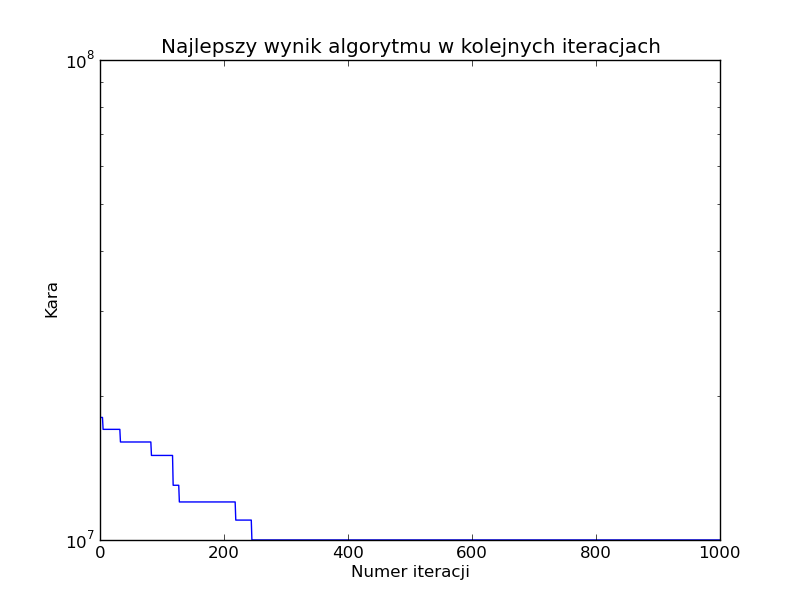
\includegraphics[width=10cm]{img/standard_penalty.png}
\centering
\end{figure}
\par Aby sprawdzić co się dzieje przyjrzałem się zachowaniu pojedynczej cząsteczki. Okazało się, że kara za kolejno generowane plany oscyluje wokół kary wyliczonej dla początkowego planu. Pokazuje to poniższy wykres.  
\begin{figure}[H]
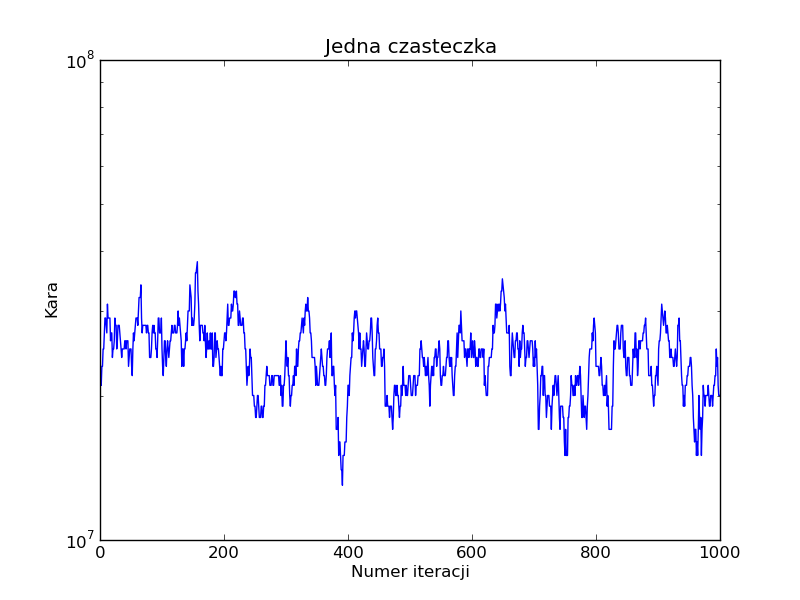
\includegraphics[width=10cm]{img/standard_particle.png}
\centering
\end{figure}
\par Na podstawie dalszej analizy okazało się, że wszystkie cząsteczki zachowują się bardzo podobnie. Widać to na poniższym wykresie.
\begin{figure}[H]
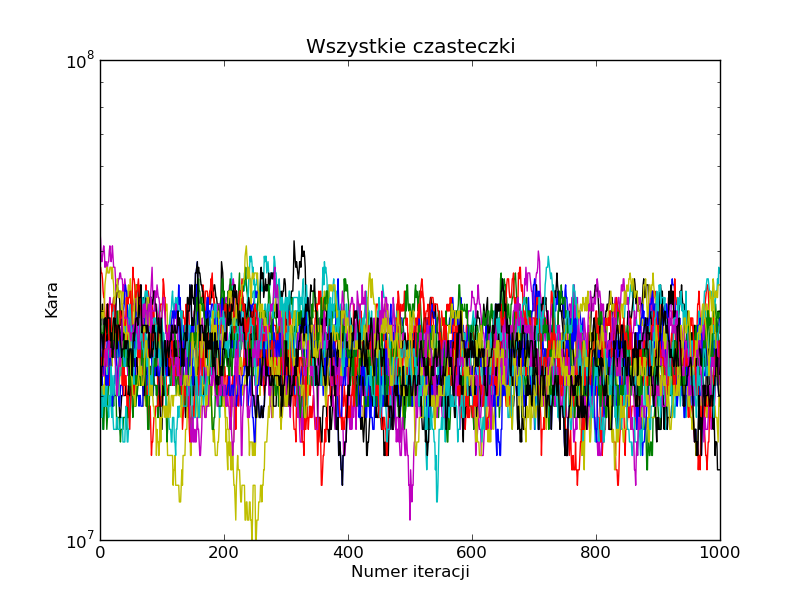
\includegraphics[width=10cm]{img/standard_particle_all.png}
\centering
\end{figure}
\subsubsection{Rozważane modyfikacje}
\par Rozważyłem dwie modyfikacje do aktualnego algorytmu. Jedną nazwałem podążaniem za lokalnie najlepszym planem, a drugą podążanie za globalnie najlepszym planem. Obie modyfikacje są względem siebie analogiczne, a różnią się tylko tym który plan bierzemy pod uwagę. Modyfikacją została objęta faza oceny aktualnego rozwiązania, która zachodzi na początku każdej iteracji. Dodany został warunek, że jeśli aktualny plan jest gorszy od najlepszego planu to zostaje on zamieniony na najlepszy plan. Usunięte też zostały kroki 3 i 4 czyli kopie z najlepszych planów.
\par W przypadku gdy każda cząsteczka podąża za swoim lokalnie najlepszym planem istnieje mniejsze ryzyko, że algorytm utknie w minimum lokalnym przestrzeni rozwiązań. Natomiast podczas podążania za globalnie najlepszym planem algorytm będzie znacznie szybciej dążył do najbliższego minimum.
\par Opcja podążania za lokalnie najlepszym planem okazała się być dużo efektywniejsza od podstawowego algorytmu. W tym przypadku ograniczenia "twarde" nie stanowiły problemu. Można to zobaczyć na poniższym wykresie.
\begin{figure}[H]
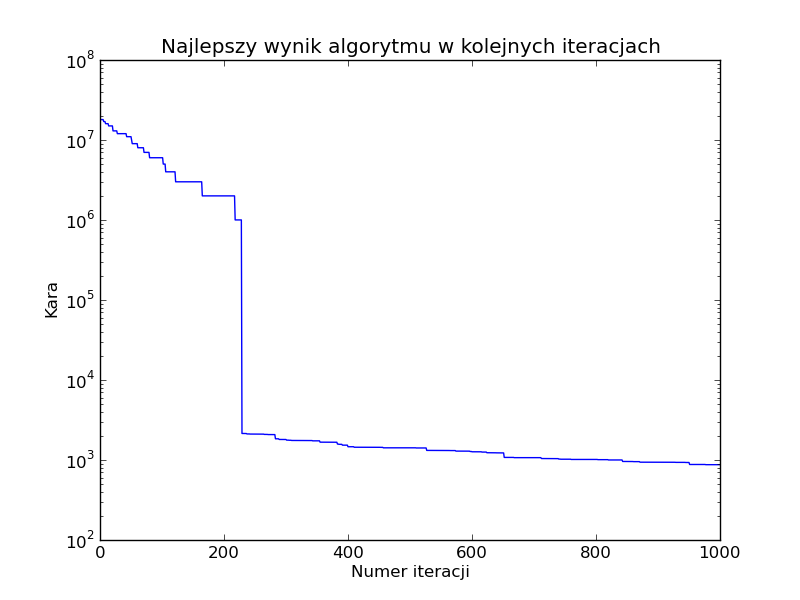
\includegraphics[width=10cm]{img/localbest_penalty.png}
\centering
\end{figure}
\par Analizując pojedynczą cząsteczkę można zauważyć, że często kara skacze od małych wartości do wartości milionowych. Jest to spowodowane tym, że w po zamianie dwóch lekcji w poprzedniej iteracji pojawił się konflikt z ograniczeniami "twardymi". Nie stanowi to problemu, ponieważ w takim przypadku wracamy do poprzedniego rozwiązania. Na poniższych wykresach widać zachowanie dla pojedynczej cząsteczki oraz dla wszystkich cząsteczek.
\begin{figure}[H]
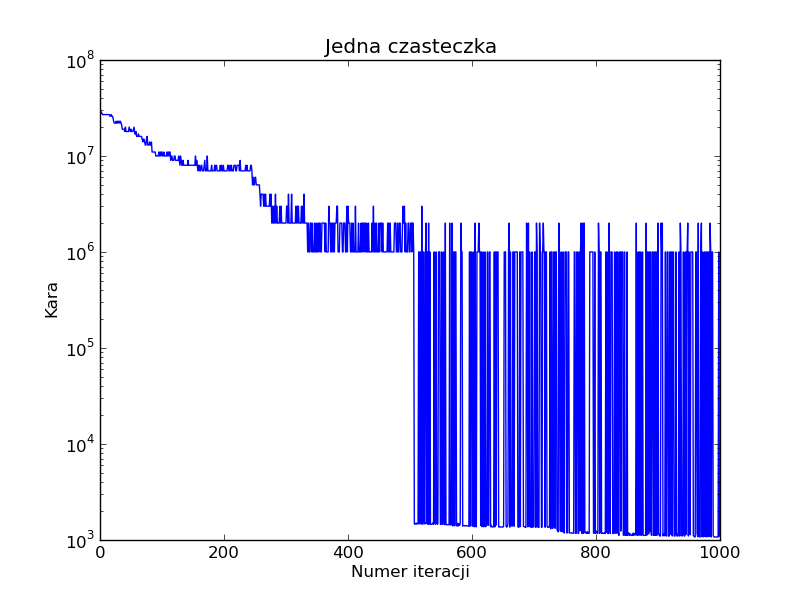
\includegraphics[width=10cm]{img/localbest_particle.png}
\centering
\end{figure}
\begin{figure}[H]
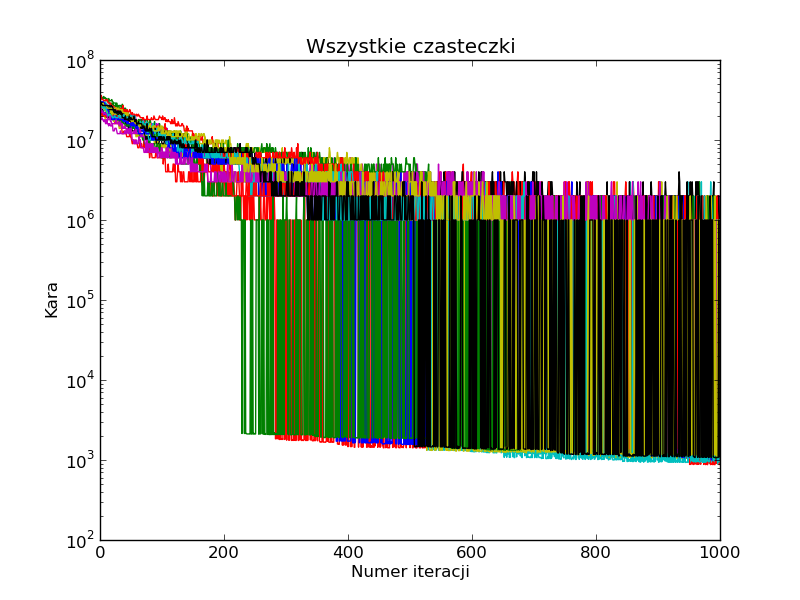
\includegraphics[width=10cm]{img/localbest_particle_all.png}
\centering
\end{figure}
\par Opcja podążania za globalnie najlepszym planem okazała się jeszcze bardziej efektywna. Sporym zaskoczeniem był brak problemów z lokalnymi minimami przestrzeni rozwiązań. Poniższy wykres pokazuje skuteczność modyfikacji.
\begin{figure}[H]
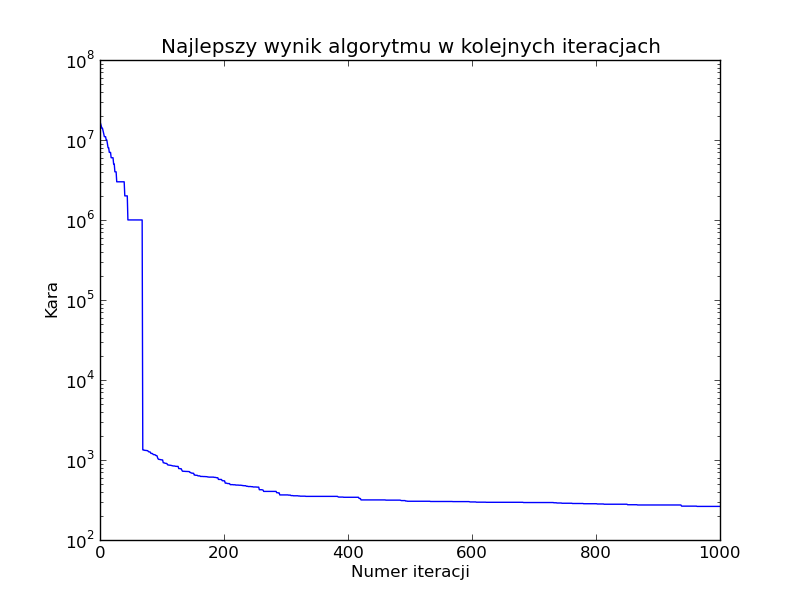
\includegraphics[width=10cm]{img/globalbest_penalty.png}
\centering
\end{figure}
\par W tym przypadku cząsteczki zachowywały się bardzo podobnie. Jedyną różnicą była prędkość z jaką spadała kara. Widać to na poniższych wykresach. 
\begin{figure}[H]
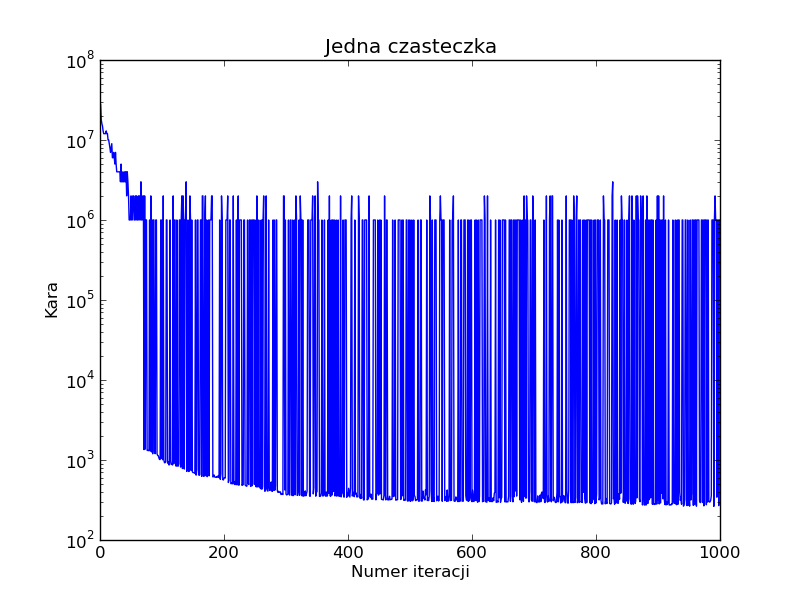
\includegraphics[width=10cm]{img/globalbest_particle.png}
\centering
\end{figure}
\begin{figure}[H]
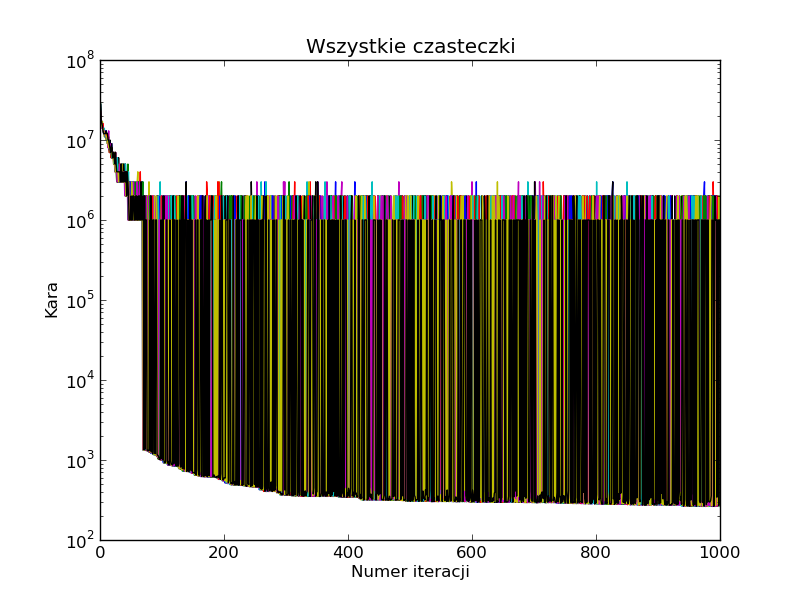
\includegraphics[width=10cm]{img/globalbest_particle_all.png}
\centering
\end{figure}
\subsubsection{Ostateczne rozwiązanie}
\par Jako ostateczne rozwiązanie wybrałem podążanie za globalnie najlepszym planem. Jest to spowodowane tym, że mimo wielu testów nie udało mi się znaleźć przypadku kiedy podążanie za lokalnie najlepszym planem wypadłoby lepiej. 
